% *********************************************************************
% © 2016–2025 Jeremy Sylvestre
%
% Permission is granted to copy, distribute and/or modify this document
% under the terms of the GNU Free Documentation License, Version 1.3 or
% any later version published by the Free Software Foundation; with no
% Invariant Sections, no Front-Cover Texts, and no Back-Cover Texts. A
% copy of the license is included in the appendix entitled “GNU Free
% Documentation License” that appears in the output document of this
% PreTeXt source code. All trademarks™ are the registered® marks of
% their respective owners.
%
% *********************************************************************
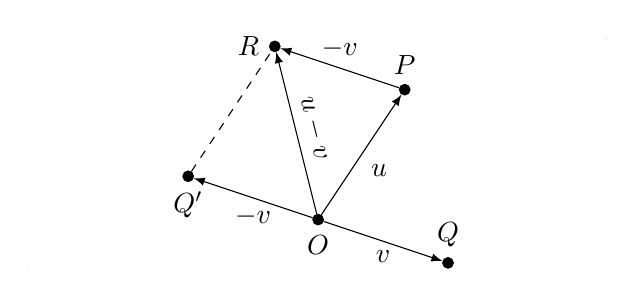
\begin{tikzpicture}[
	point/.style={circle,draw,very thin,fill,inner sep=0pt,minimum size=4pt},
	vector/.style={-latex},
	scale=0.55
]

	% want to artificially widen image because its in a sidebyside with a <p>
	% and want caption to be wider
	%
	% actual image dimensions: from (-3.25,-1.1) to (3.2,4.2)
	%
	\draw[black!5!white,very thin] (-6.7,-1.05) to (-6.7,-1.1) to (-6.65,-1.1);
	\draw[black!5!white,very thin] (6.65,4.15) to (6.65,4.2) to (6.6,4.2);

	\node[point] at (0,0) (o) [label=below:{$O$}] {};
	\node[point] at (2,3) (p) [label=above:{$P$}] {};
	\node[point] at (3,-1) (q) [label=above:{$Q$}] {};
	\node[point] at (-3,1) (q2) [label=below:{$Q'$}] {};
	\node[point] at (-1,4) (r) [label=left:{$R$}] {};
	\draw[vector] (o) to node[below right] {$\uvec{u}$} (p);
	\draw[vector] (o) to node[below] {$\uvec{v}$} (q);
	\draw[vector] (o) to node[below] {$-\uvec{v}$} (q2);
	\draw[vector] (p) to node[above] {$-\uvec{v}$} (r);
	\draw[vector] (o) to node[sloped,above] {$\uvec{u}-\uvec{v}$} (r);
	\draw[dashed] (q2) to (r);
\end{tikzpicture}
